\state{Spacetime diagrams (MCP 2.14)}{ \label{4}
	Use spacetime diagrams to prove the following.
}

\begin{figure}[p] \centering
	\begin{tabular}{c@{\hspace{0.5in}} c}
		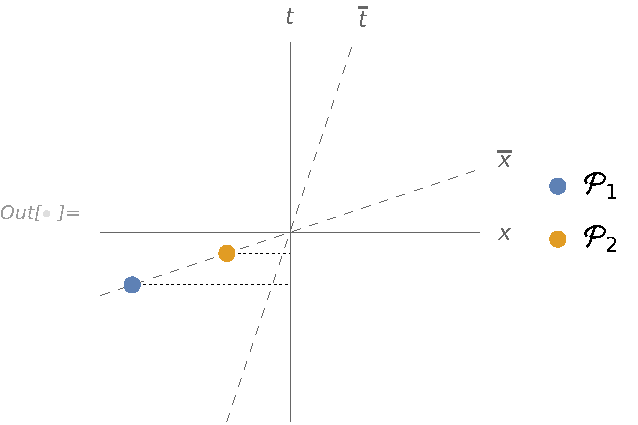
\includegraphics[trim=1.5cm 0 0 0,clip,width=0.4\textwidth]{4a} &
		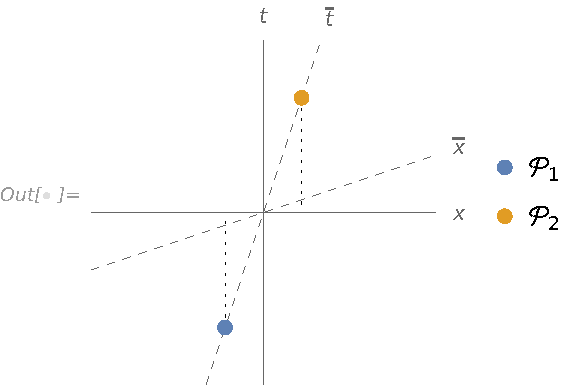
\includegraphics[trim=1.5cm 0 0 0,clip,width=0.4\textwidth]{4b} \\
		(a) & (b) \\[0.5in]
		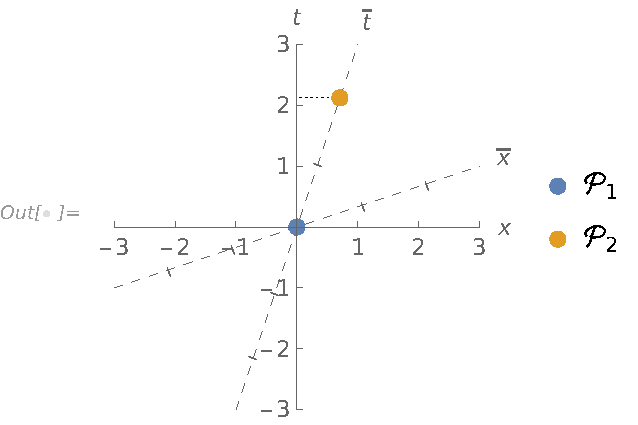
\includegraphics[trim=1.5cm 0 0 0,clip,width=0.4\textwidth]{4c} &
		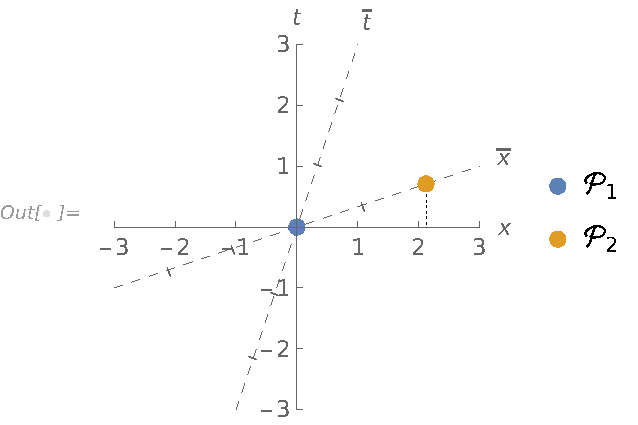
\includegraphics[trim=1.5cm 0 0 0,clip,width=0.4\textwidth]{4d} \\
		(c) & (d) \\[0.5in]
		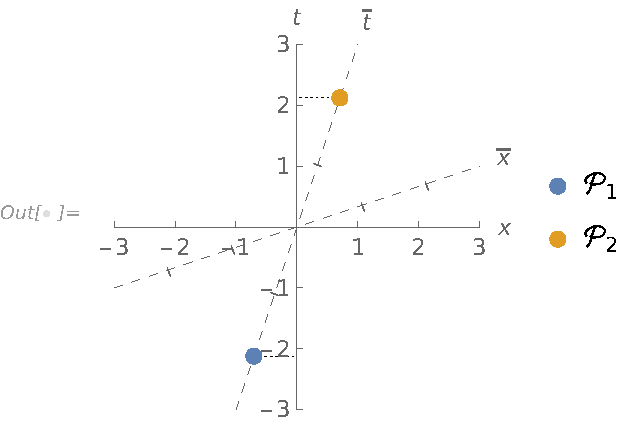
\includegraphics[trim=1.5cm 0 0 0,clip,width=0.4\textwidth]{4e} &
		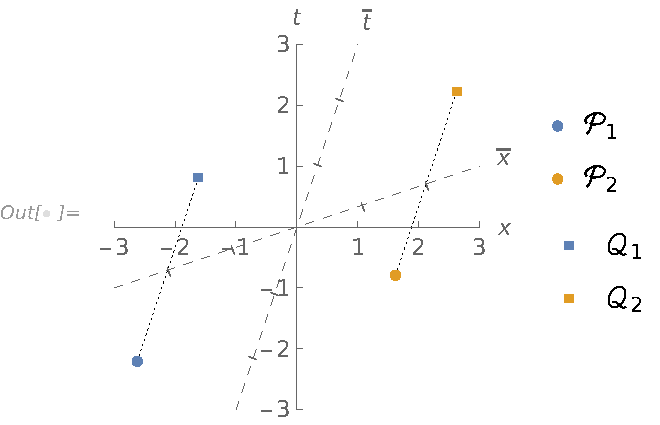
\includegraphics[trim=1.5cm 0 0 0,clip,width=0.4\textwidth]{4f} \\
		(e) & (f) \\
	\end{tabular}
	\caption{Spacetime diagrams for problems~\ref{4}.}
	\label{f4}
\end{figure}

\prob{
	Two events that are simultaneous in one inertial frame are not necessarily simultaneous in another.  More specifically, if frame $\cFb$ moves with velocity $\vv = \bet \vex$ as seen in frame $\cF$, where $\bet > 0$, then of two events that are simultaneous in $\cFb$ the one farther ``back'' (with the more negative value of $\xb$) will occur in $\cF$ before the one farther ``forward.''
}

\sol{
	Figure~\ref{f4}~(a) shows a spacetime diagram for frames $\cF$ and $\cFb$.  Two events, $\cPq$ and $\cPw$, are located on the $\xb$ axis.  In $\cFb$, they occur simultaneously at $\tb = 0$.  The dotted lines extending from the events to the $t$ axis show when the events occur in $\cF$.  Event $\cPq$ is farther back and occurs earlier in $\cF$ than event $\cPw$.  Thus two events that are simultaneous in $\cFb$ are not simultaneous in $\cF$. \qed
}



\prob{
	Two events that occur at the same spatial location in one inertial frame do not necessarily occur at the same spatial location in another.
}

\sol{
	Figure~\ref{f4}~(b) shows a spacetime diagram in which events $\cPq$ and $\cPw$ both occur at position $\xb = 0$ in $\cFb$.  The dotted lines extending from the events to the $x$ axis show that, in $\cF$, event $\cPq$ occurs at $x < 0$ and event $\cPw$ at $x > 0$.  Hence, the events do not occur at the same position in $\cF$. \qed
}



\prob{
	If $\cPq$ and $\cPw$ are two events with a timelike separation, then there exists an inertial reference frame in which they occur at the same spatial location, and in that frame the time lapse between them is equal to the square root of the negative of their invariant interval, $\Del t = \Del \tau \equiv \sqrt{-(\Del s)^2}$.
}

\sol{
	Figure~\ref{f4}~(c) shows a spacetime diagram in which axes are given arbitrary units.  Events $\cPq$ and $\cPw$ occur at the same location in $\cF$, $x = 2$.  The dotted lines show the $(\tb, \xb)$ coordinates of $\cPq$ and $\cPw$.  The interval is clearly timelike as viewed from $\cFb$ since $\Del\tb > \Del\xb$.  Since the interval is invariant of reference frame, it can be calculated in one spatial and one temporal dimension by adapting (2.2a) in MCP:
	\eqn{interval}{
		(\Del s)^2 = -(\Del t)^2 + (\Del x)^2.
	}
	In $\cF$, $\Del x = 0$ and $\Del t = 1$.  Then
	\eq{
		(\Del s)^2 = -1^2 + 0^2
		= -1
		< 0,
	}
	so the interval is indeed timelike~\cite[p.~45]{MCP}.  Since the events are at the same spatial location in $\cF$, we calculate the time lapse between them in $\cF$ as
	\eq{
		\sqrt{-(\Del s)^2} = \sqrt{1} = 1,
	}
	which is exactly as shown in Fig.~\ref{4}~(c). \qed
}



\prob{
	If $\cPq$ and $\cPw$ are two events with a spacelike separation, then there exists an inertial reference frame in which they are simultaneous, and in that frame the spatial distance between them is equal to the square root of their invariant interval, $\sqrt{\gij \Del \xii \Del \xj} = \Del s \equiv \sqrt{(\Del s)^2}$.
}

\sol{
	Figure~\ref{f4}~(d) shows a spacetime diagram in which events $\cPq$ and $\cPw$ have a spacelike separation.  The dotted lines show the $(\tb, \xb)$ coordinates of $\cPq$ and $\cPw$.  The interval is obviously spacelike as viewed from $\cFb$ because $\Del\tb < \Del\xb$.  In $\cF$, the events occur simultaneously at $t = 2$, and $\Del x = 1$, $\Del t = 0$.  Using Eq.~\refeq{interval} to compute the interval, we find
	\eq{
		(\Del s)^2 = -0^2 + 1^2
		= 1
		> 0,
	}
	so the interval is indeed spacelike~\cite[p.~45]{MCP}.  Since the events are simultaneous in $\cF$, we calculate the spatial distance between them as
	\eq{
		\sqrt{(\Del s)^2} = \sqrt{1} = 1,
	}
	which is exactly as shown in Fig.~\ref{4}~(d). \qed
}



\prob{
	If the inertial frame $\cFb$ moves with speed $\bet$ relative to the frame $\cF$, then a clock at rest in $\cFb$ ticks more slowly as viewed from $\cF$ than as viewed from $\cFb$---more slowly by a factor $\gam^{-1} = \sqrt{1 - \bet^2}$.  This is called \emph{relativistic time dilation}.  As one consequence, the lifetimes of unstable particles moving with a speed $\bet$ are increased by the Lorentz factor $\gam$.
}

\sol{
	Figure~\ref{f4}~(e) shows a spacetime diagram in which $\cPq$ represents a tick of a clock and $\cPw$ the clock's subsequent tick.  Both events occur at $\xb = 0$, so the clock is stationary in $\cFb$.  $\cPq$ occurs at $\tb = -2$ and $\cPw$ occurs at $\tb = 2$.  In $\cFb$, the time between ticks is $\Del\tb = 4$; in $\cF$, the dotted lines indicate that $\Del t > 4$.  In this figure
	\aln{ \label{gambet}
		\bet &= \frac{1}{3}, &
		\gam &= \frac{3}{2 \sqrt{2}} \approx 1.06.
	}
	So in $\cF$, the time between ticks is $\Del t = 4\gam \approx 4.24$.  The dotted lines indeed intersect the $t$ axis at $t = \pm 2 \gam \approx \pm 2.12$, which confirms time dilation. \qed
}



\prob{
	If the inertial frame $\cFb$ moves with velocity $\vv = \bet \vex$ relative to the frame $\cF$, then an object at rest in $\cFb$ as studied in $\cF$ appears shortened by a factor $\gam^{-1} = \sqrt{1 - \bet^2}$ along the $x$ direction, but its length along the $y$ and $z$ directions is unchanged.  This is called \emph{Lorentz contraction}.  As one consequence, heavy ions moving at high speeds in a particle accelerator appear to act like pancakes, squashed along their directions of motion.
}

\sol{
	Figure~\ref{f4}~(f) shows a spacetime diagram in which a rod at rest in $\cFb$ has endpoints located at $\cPq, \cPw$.  The dotted lines represent the worldlines of the ends of the rod as time passes and the rod moves in the $x$ direction with velocity $\vv = \vex / 3$.  After some length of time has passed, the ends of the rod are located at $\cQq, \cQw$, but its position in $\cFb$ has not changed.
	
	The length of the rod in $\cFb$ is $\Del\xb = 4$.  The length of the rod in $\cF$, $\Del x$, is the distance between the points at which the worldlines intersect the $x$ axis.  Clearly $\Del x < 4$.  Applying Eq.~\refeq{gambet} once more, we see that $\Del x = 4 / \gam \approx 3.77$.  The worldlines intersect the $x$ axis at $x = \pm 1.89$, which confirms length contraction~\cite[p.~194]{Resnick}.
	
	An observer in $\cF$ does not see the rod move in the $y$ or $z$ directions.  Therefore special relativity is not relevant when considering these directions, so the length of the rod in the $y$ and $z$ directions is the same in $\cF$ as it is in $\cFb$. \qed
}